We are going to make a short introduction to what neural networks and deep learning are, with particular reference to networks architectures we are going to exploit in the next chapters.

The primary objective of deep learning methods is to find a function that maps an input to an output in an "optimal" way (i.e., minimizing some cost function). Deep learning methods are particularly useful when the structure of the optimal solution is not known, but there is an ample dataset of "correct" examples.

The strategy to solve them is always the same: 
\begin{enumerate}
    \item Choose a differentiable parametric function $\hat{y} = f(x,p)$, where $x$ is the input and $p$ the parameters;
    \item Define a differentiable loss function $L(\hat{y})$ and minimize it with respect to $p$ (using its derivatives);
    \item Compute derivatives of $L$ with respect to $p$ and use them to find optimal parameters.
\end{enumerate}

The choice of the function $f$ is the difficult point and a fundamental goal of this work. There are different architectures we can use to develop a good model:
\begin{itemize}
    \item Dense neural networks (multilayer perceptron);
    \item Convolutional neural networks;
    \item Recurrent neural networks.
\end{itemize}

\section{Dense neural networks (multilayer perceptron)}
Dense Neural Network (DNN), which is the simplest neural network architecture, is a biologically inspired computational model. Its layers are densely connected, which means each neuron in a layer receives an input from all the neurons in the previous layer (i.e., each neuron is connected to all neurons of the previous layer) and similarly, it is an input for all the neurons in the following layers, as we can see in Figure~\ref{fig:DNN}.

\begin{figure}[H]
    \centering
    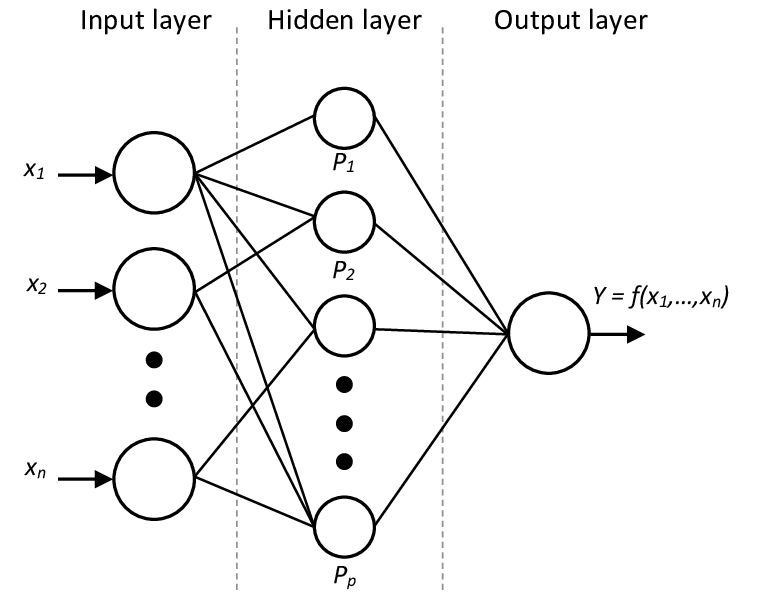
\includegraphics[width=0.6\textwidth]{Images/DNN.png}
    \caption{Dense neural network}
    \label{fig:DNN}
\end{figure}


\section{Convolutional neural networks}
A dense architecture is really simple to understand, but it ignore the structure of the problem at hand. The knowledge about the structure of natural images suggests two key principles to prevent the explosion in the number of parameters:
\begin{enumerate}
    \item \textbf{Locality:} each pixel should only received inputs from nearby pixels;
    \item \textbf{Equivariance:} a shift in the input image should correspond to a shift in the output image.
\end{enumerate}


The convolution formula with input channels $C_1$ and output channels $C_2$ is:
\begin{equation}
    J[i_1,i_2,c_2] = \sum_{c_1 \in C_1}\sum_{k_1 \in K_1}\sum_{k_2 \in K_2}{W[k_1, k_2, c_1, c_2]I[i_1 - k_1, i_2 - k_2, c_1]}
\end{equation}


\begin{figure}[H]
    \centering
    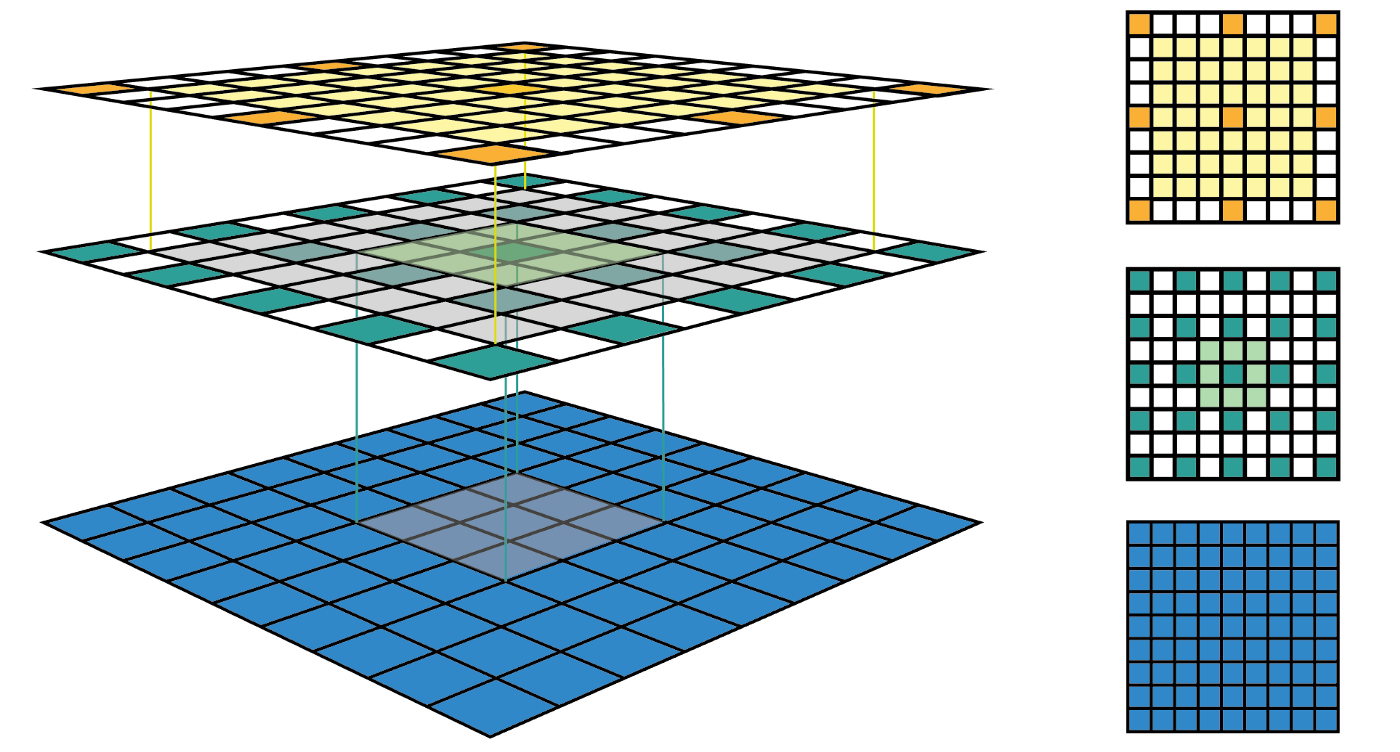
\includegraphics[width=0.7\textwidth]{Images/CNN_filter.png}
    \caption{Convolutional neural network}
    \label{fig:CNN_filter}
\end{figure}


\section{Recurrent neural networks}
Recurrent neural networks (RNN) was developed to work with sequential data. Data are sequential when their underlying temporal dynamics is more relevant than the information carried by each individual data point. 

The idea under RNN is to add knowledge of the immediate past to the current state of the network allowing output from some nodes to affect subsequent input to the same nodes (graphically, connections between nodes can create a cycle).

\begin{figure}[H]
    \centering
    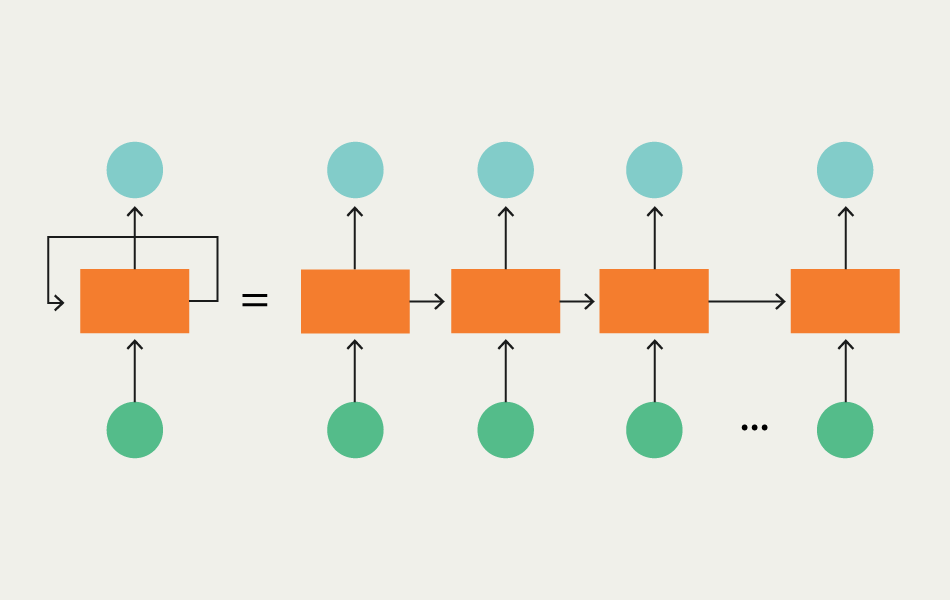
\includegraphics[width=0.7\textwidth]{Images/RNN.png}
    \caption{Recurrent neural network}
    \label{fig:RNN}
\end{figure}

